%!TEX root = ../report.tex

% 
% Architecture
% 

\section{Architecture (2/3pgs)}
\label{sec:arch}

As discussed in the previous section, the general purpose programming environments provide advanced features for editing, refactoring and debugging code, but the representation of code in those editors are purely textual and most of time the code must be compiled and executed manually. On the other hand, the environments used in generative design, for instance, provide straightforward features for beginners, but does not suite well as program grows.

The problem addressed in this work is to design and implement an interactive programming environment. Our approach suggests two features. The first, illustrates the code with program's sketches improving the program documentation. The second, allows the result of the code be visualized as soon as possible improving the program comprehension. More important than these features, are the underlying design principles that they represent, and understand how these principles enable the programmer to think.

The features we propose will be built on top of DrRacket~\cite{findler2002drscheme}. In the following sections, we will present relevant properties of DrRacket that justify its choice as the basis of this work, as well as the proposed architecture to extend the DrRacket environment.

\subsection{DrRacket Properties}

Like DrRacket, our solution initially will target at students. The features, we propose, are supposed to be used for quickly experiment ideas and progressively migrate these experiments to a bigger project. However, this interactive environment can be used for either beginner which wants to understand a piece of code or a professional programmer which needs to test a particular module.

DrRacket was built in the same principle we search for and has some key qualities:

\begin{itemize}
	\item \textbf{Pedagogic.} DrRacket has been a popular environment for introductory courses in programming languages. The environment is designed to guide the student by catching typical mistakes and explain them in terms the students understand. The environment is also useful for professional programmers, due to its sophisticated programming tools, such as the static debugger, and its advanced language features, such as units and mixins.

	\item \textbf{Sophisticated editor.} DrRacket fully integrates a graphics-enriched editor which supports, in addition to plain text, elements such as images, boxes (with comments, Racket code and XML code), etc. DrRacket also displays these elements appropriately in the read-eval-print loop.

	\item \textbf{Extensible.} The main features of DrRacket environment was implemented on top of tools. For example, the debugger, the syntax checker and the stepper are implemented as tools. Despite these tools provide different functionalities, all of them share the same API. And this API is available for any ordinary tool.
\end{itemize}

However, DrRacket lacks on a mechanism which enables beginner programmers to effortless read the code and also allow them immediately see the result of their actions. In the next section, we present a possible way to integrate these mechanisms in DrRacket.

\subsection{Proposed Architecture}

The Figure~\ref{fig:solution} present a publish-subscribe view of the proposed tool. There are two different interactions in this architecture, the first presented by a publish-subscribe and the second by a client-server.

\begin{enumerate}
	\item \texttt{DrRacket UI event manager} acts as an event bus for user-interface events (such as button clicks). Subscription information, i.e. what UI events are relevant to our system and what components handle them, is defined at load time when the event manager reads the plugin configuration file, in this case the \texttt{info} file. So, when user are working on a editor, an UI event is generated and dispatched via implicit invocation to the action handler objects that subscribe to that event.

	\item The manuscripts symbols, present on the image, will be parsed using an optical character recognition (OCR) engine. We expect the OCR acts as an external service providing a service to identify those symbols. For this purpose, in our architecture the \texttt{symbol identifier} component call the service while handle the recognition of the image.
\end{enumerate}

\begin{figure}[htb]
	\centering
	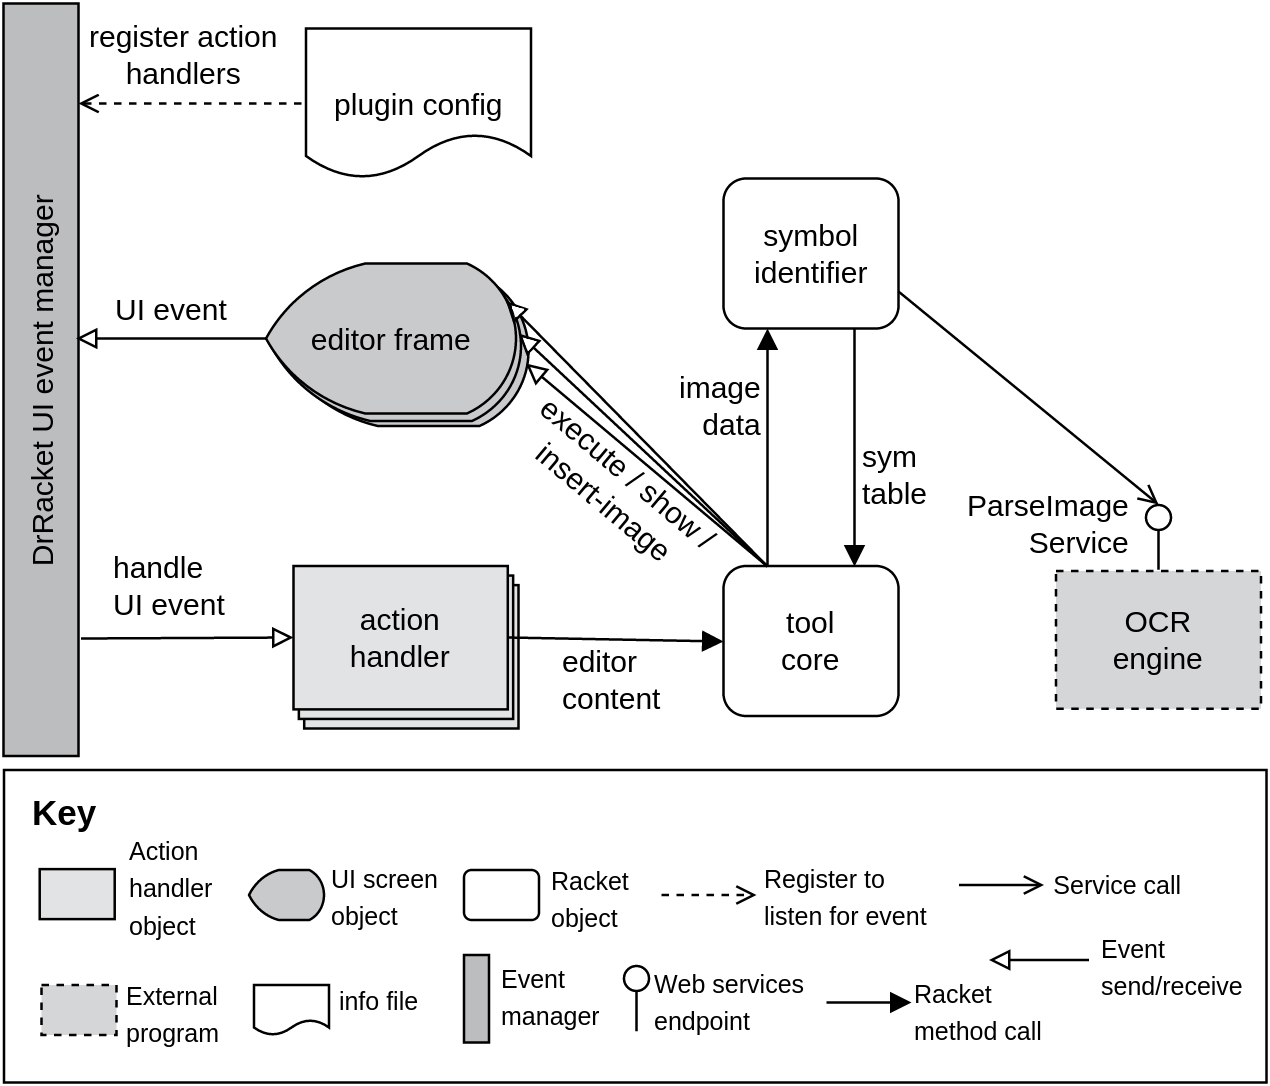
\includegraphics[scale=0.19]{img/solution}
	\caption{Diagram for a publish subscribe view of the proposed architecture.}
	\label{fig:solution}
\end{figure}

The \texttt{tool core} component, in Figure~\ref{fig:solution}, will change the editor based on, mainly, the following events:

\begin{itemize}
	\item \texttt{on-change:} when DrRacket detects that the editor has been modified, it sends the contents of the editor over to action handlers.
	The action handler, in this case is the \texttt{online expansion handler} an separated place where the code are expanded. \textit{Desired action}: \texttt{execute} the code when the syntax is correct. 

	\item \texttt{on-paint:} this event is sent just before and just after every painting of the editor. Handling this event provide a way to add arbitrary graphics to an editor's display. \textit{Desired action}: \texttt{show} a slider widget when the cursor stops over a literal.

	\item \texttt{on-new-image-snip:} this event is sent when an image is inserted in the editor. The default implementation creates an image snip which is an object with the image information, such as path, format, etc. \textit{Desired action}: get the image and sent it to the OCR engine to recognize its symbols and respective coordinates (x, y). Then return an subclass of image snip, adding this extra information.
\end{itemize}

Finally, to extend the arrow mechanism of DrRacket we will use an syntactic transformer, i.e. macro. The macro will add in the AST bound occurrences of the function's parameter. As a result, the DrRacket arrow mechanism will be able to recognize bound occurrences and point to them inside an image.